\documentclass[12pt]{article}
\usepackage[spanish]{babel}
\usepackage[utf8]{inputenc}
\usepackage{graphicx}
\usepackage{amsmath}
\usepackage{booktabs}
\usepackage{float}
\usepackage{hyperref}
\usepackage[ruled,vlined]{algorithm2e}

\title{Taller 3a – Preparación de Datos y Modelos Predictivos}
\author{Estudiante: Juan Felipe Gómez Carmona \\ 
Maestría en Analítica Aplicada \\
Universidad de La Sabana \\ 
Profesor: Hugo Franco, Ph.D.}
\date{Octubre 2025}

\begin{document}

\maketitle
\tableofcontents
\newpage

\section{Introducción}
El presente taller tiene como objetivo aplicar los principios del flujo de trabajo de Ciencia de Datos en la preparación, imputación y modelado de conjuntos de datos con valores faltantes. 
A partir del \textit{Cleveland Heart Disease Dataset}, se busca evaluar el impacto de distintas estrategias de imputación en el rendimiento de modelos supervisados, así como comparar dos algoritmos ampliamente usados en clasificación: \textbf{Random Forest} y \textbf{XGBoost}.

\section{Metodología}

\subsection{Dataset y Preprocesamiento}
Se emplearon dos datasets:
\begin{itemize}
    \item \textbf{Penguins Dataset}: utilizado para practicar la creación de \textit{pipelines} con imputación, escalamiento y detección de valores atípicos.
    \item \textbf{Cleveland Heart Disease Dataset}: empleado para evaluar el impacto de diferentes estrategias de imputación y comparar modelos de clasificación.
\end{itemize}

En el conjunto de Cleveland, compuesto por 303 registros y 14 atributos clínicos, las columnas \texttt{ca} y \texttt{thal} presentaban valores faltantes, los cuales fueron convertidos a \texttt{NaN} para su imputación posterior.  

\subsection{Estrategias de Imputación}
Se evaluaron distintas estrategias mediante \texttt{SimpleImputer} y \texttt{KNNImputer}, integradas en un pipeline junto con estandarización (\texttt{StandardScaler}) y el clasificador correspondiente.  
Las estrategias incluyeron:
\begin{itemize}
    \item \textbf{mean}: reemplazo por la media de la columna.
    \item \textbf{median}: reemplazo por la mediana.
    \item \textbf{most\_frequent}: reemplazo por el valor más frecuente.
    \item \textbf{constant}: reemplazo por un valor fijo (0).
    \item \textbf{KNN}: imputación basada en vecinos más cercanos ($k=5$).
\end{itemize}

\subsection{Comparación de Modelos}
Luego de determinar la mejor estrategia de imputación, se compararon los modelos \textbf{Random Forest} y \textbf{XGBoost}.  
El flujo de procesamiento incluyó:
\begin{enumerate}
    \item Imputación con el método \textit{constant} (reemplazo por 0).
    \item Estandarización con \texttt{StandardScaler}.
    \item Entrenamiento de los clasificadores sobre el conjunto de entrenamiento.
    \item Evaluación mediante métricas de \textit{accuracy}, \textit{recall} y \textit{precision}.
\end{enumerate}

\subsection*{Cómo ejecutar y archivos entregados}
Los scripts entregados están disponibles en GitHub (\texttt{taller3-ml-analisis}).  
Para replicar los resultados:
\begin{enumerate}
    \item Crear un entorno virtual e instalar dependencias:
\begin{verbatim}
python -m venv .venv
source .venv/bin/activate   # (Windows: .venv\Scripts\activate)
pip install -r requirements.txt
\end{verbatim}
    \item Ejecutar:
\begin{verbatim}
python data_prep.py
\end{verbatim}
    \item Las figuras generadas se almacenan en la carpeta \texttt{figures/}.
\end{enumerate}

\subsection*{Algoritmo del pipeline propuesto}
\begin{algorithm}[H]
\caption{Pipeline de preparación e imputación}
\KwIn{Datos clínicos $X$, etiquetas $y$}
\KwOut{Modelo entrenado $\mathcal{M}$ y métricas}
Dividir $X,y$ en entrenamiento y prueba (stratificado)\;
Imputar valores faltantes (\texttt{constant}/\texttt{median}/\texttt{KNN})\;
Estandarizar con \texttt{StandardScaler}\;
Entrenar clasificador (\texttt{RandomForest} o \texttt{XGBoost})\;
Evaluar con \texttt{accuracy}, \texttt{recall}, \texttt{precision}\;
\Return $\mathcal{M}$ y métricas\;
\end{algorithm}

\section{Resultados}

\subsection{Validación con el dataset Penguins}
Como se observa en la Figura~\ref{fig:penguins-cm}, el modelo logra clasificar correctamente las especies del dataset original.  
Tras aplicar la técnica de \textit{capping} de valores atípicos (Figura~\ref{fig:penguins-cap}), el desempeño se mantiene estable con una exactitud superior al 95\%.

\begin{figure}[H]
\centering
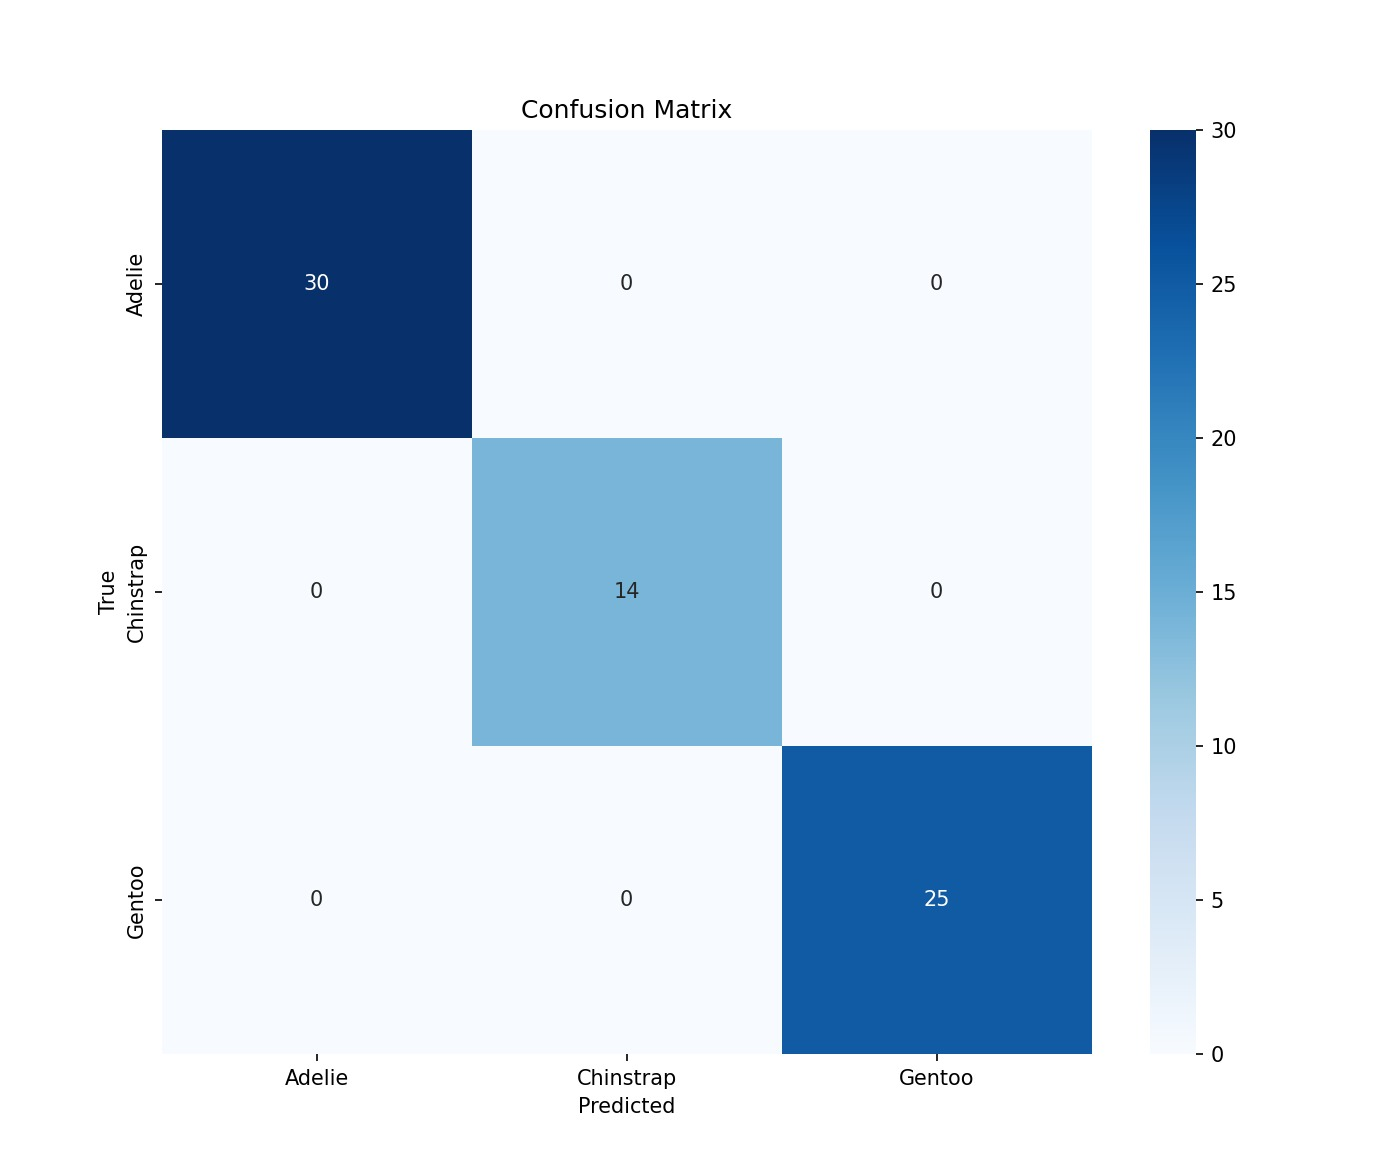
\includegraphics[width=0.75\textwidth]{figures/penguins_confusion_matrix.png}
\caption{Matriz de confusión inicial del modelo en el dataset Penguins.}
\label{fig:penguins-cm}
\end{figure}

\begin{figure}[H]
\centering
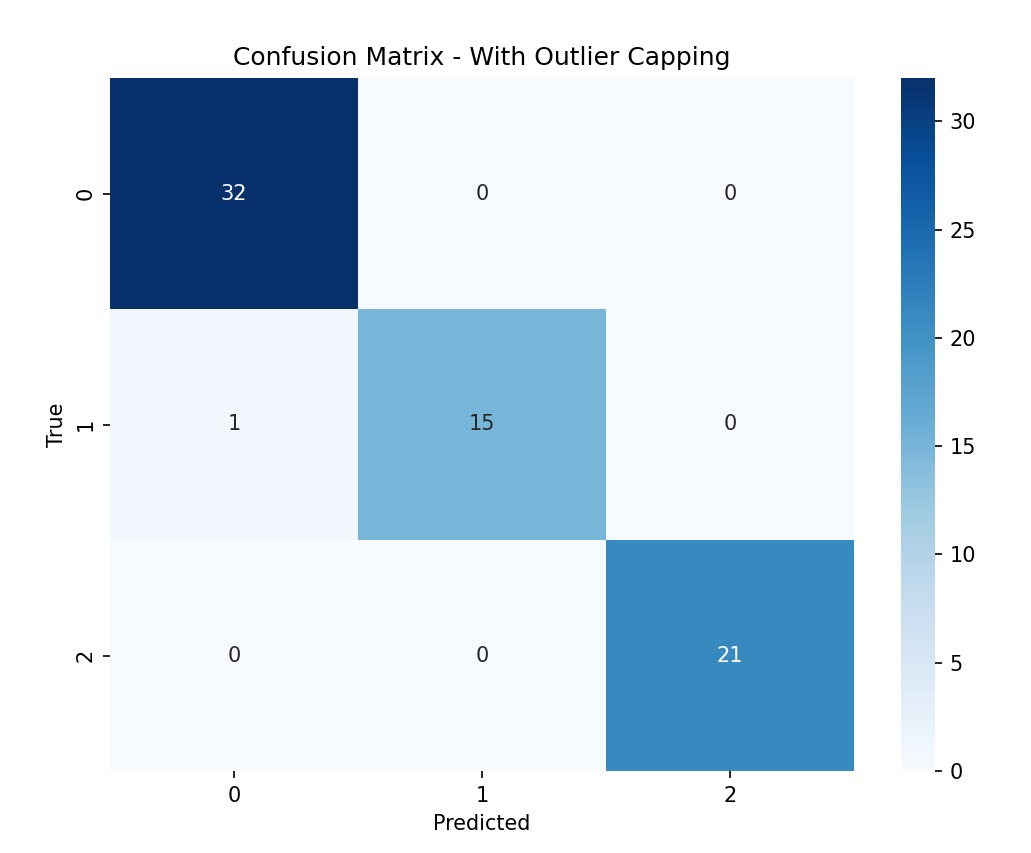
\includegraphics[width=0.75\textwidth]{figures/penguins_outlier_capping.png}
\caption{Matriz de confusión posterior al capping de valores atípicos.}
\label{fig:penguins-cap}
\end{figure}

\subsection{Impacto de la Imputación de Datos (Cleveland)}
Los resultados de las estrategias de imputación se resumen en el Cuadro~\ref{tab:imputacion}.  
La imputación \textbf{constant} alcanzó la mayor precisión (90.16\%), mientras que \textit{median} y \textit{most frequent} también ofrecieron resultados competitivos.

\begin{table}[H]
\centering
\begin{tabular}{l c}
\toprule
\textbf{Estrategia} & \textbf{Accuracy} \\
\midrule
Mean & 0.8688 \\
Median & 0.8852 \\
Most Frequent & 0.8852 \\
Constant & \textbf{0.9016} \\
KNN & 0.8688 \\
\bottomrule
\end{tabular}
\caption{Comparación del rendimiento según la estrategia de imputación.}
\label{tab:imputacion}
\end{table}

\subsection{Comparación de Modelos}
En la Tabla~\ref{tab:modelos} se comparan los resultados de ambos clasificadores.  
\textbf{Random Forest} superó a \textbf{XGBoost} en todas las métricas evaluadas.

\begin{table}[H]
\centering
\begin{tabular}{l c c c}
\toprule
\textbf{Modelo} & \textbf{Accuracy} & \textbf{Recall (Clase 1)} & \textbf{Precision (Clase 1)} \\
\midrule
Random Forest & \textbf{0.90} & 0.96 & 0.84 \\
XGBoost & 0.85 & 0.93 & 0.79 \\
\bottomrule
\end{tabular}
\caption{Comparación de desempeño entre Random Forest y XGBoost.}
\label{tab:modelos}
\end{table}

\begin{figure}[H]
\centering
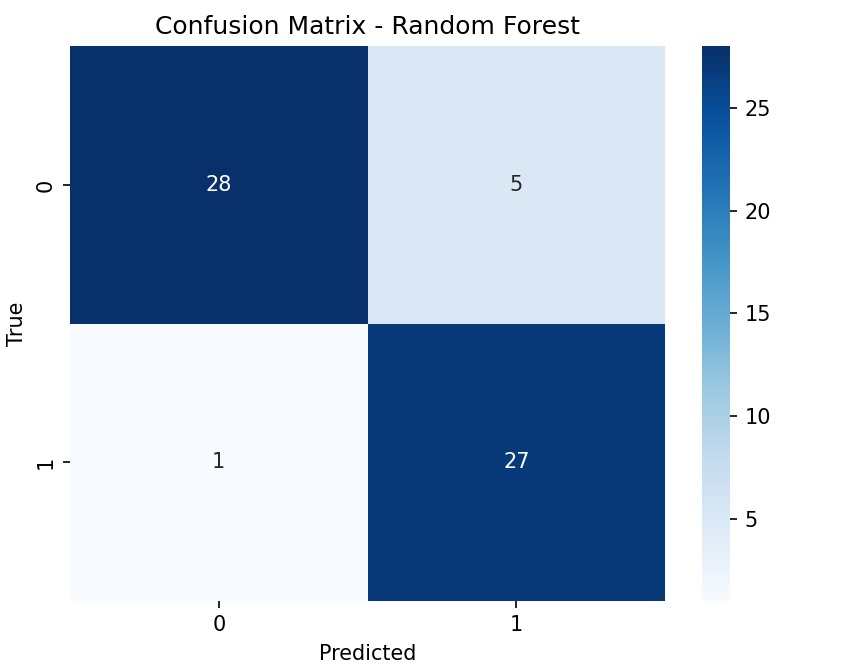
\includegraphics[width=0.7\textwidth]{figures/random_forest_confusion.png}
\caption{Matriz de confusión del modelo Random Forest.}
\label{fig:rf-cm}
\end{figure}

\begin{figure}[H]
\centering
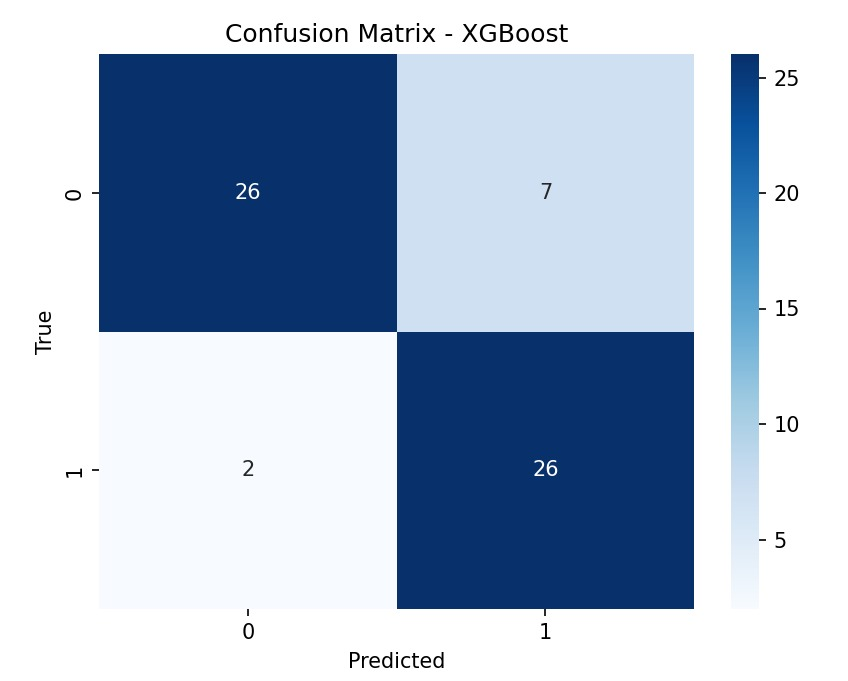
\includegraphics[width=0.7\textwidth]{figures/xgboost_confusion.png}
\caption{Matriz de confusión del modelo XGBoost.}
\label{fig:xgb-cm}
\end{figure}

\section{Discusión}
Los resultados demuestran que el proceso de preprocesamiento influye significativamente en el rendimiento final del modelo.  
El método de imputación \textbf{constant} ofreció un equilibrio adecuado entre simplicidad y desempeño.  
En cuanto a los algoritmos, \textbf{Random Forest} superó a \textbf{XGBoost} en todas las métricas, mostrando mayor estabilidad y precisión en la detección de pacientes con enfermedad.  
Este hallazgo es relevante en contextos clínicos donde el \textit{recall} es crítico para reducir falsos negativos.

\section{Conclusiones}
\begin{itemize}
    \item La imputación de valores faltantes mediante la estrategia \textbf{constant} logró la mejor precisión global (90\%).
    \item \textbf{Random Forest} se destacó por su mayor capacidad de generalización y balance entre \textit{recall} y \textit{precision}.
    \item Las diferencias en desempeño entre modelos refuerzan la importancia del preprocesamiento de datos dentro del flujo de trabajo de Machine Learning.
    \item Un pipeline bien diseñado, con imputación adecuada y estandarización, permite maximizar la efectividad de los modelos predictivos.
\end{itemize}

\section{Referencias}
\begin{itemize}
    \item UCI Machine Learning Repository. (2025). \textit{Cleveland Heart Disease Dataset}. Disponible en: \url{https://archive.ics.uci.edu/ml/machine-learning-databases/heart-disease/}
    \item Scikit-learn Documentation. (2025). \textit{Imputation and Pipelines}. Disponible en: \url{https://scikit-learn.org/stable/modules/impute.html}
    \item Chen, T., \& Guestrin, C. (2016). \textit{XGBoost: A Scalable Tree Boosting System}. KDD.
    \item Waskom, M. (2021). \textit{Seaborn: statistical data visualization}. Journal of Open Source Software, 6(60), 3021.
\end{itemize}

\end{document}
